%        File: 03140299.tex
%     Created: Fri Jan 02 03:00 PM 2015 J
% Last Change: Fri Jan 02 03:00 PM 2015 J
%
\documentclass[10pt,a4paper,twocolumn]{jarticle}

%%%%%%%%%%%%%%%%%%%%%
% to input Japanese %
%%%%%%%%%%%%%%%%%%%%%
\usepackage[japanese]{babel}

%%%%%%%%%%%%%%%%%%%%%
% to insert itembox %
%%%%%%%%%%%%%%%%%%%%%
\usepackage{ascmac}

%%%%%%%%%%%%%%%%%%%%%%%%%%
% to be standard a4paper %
%%%%%%%%%%%%%%%%%%%%%%%%%%
\usepackage{geometry}
\geometry{
  a4paper,
  total={210mm,297mm},
  left=20mm,
  right=20mm,
  top=20mm,
  bottom=40mm,
}

%%%%%%%%%%%%%%%%%%%%%
% to insert figures %
%%%%%%%%%%%%%%%%%%%%%
\usepackage[dvipdfmx]{graphicx}

%%%%%%%%%%%%%%%%%%%%%%%%%%
% to insert source codes %
%%%%%%%%%%%%%%%%%%%%%%%%%%
% \usepackage{listings, jlisting}
% \renewcommand{\lstlistingname}{list}
% \lstset{language=C,
%   basicstyle=\ttfamily\scriptsize,
%   commentstyle=\textit,
%   classoffset=1,
%   keywordstyle=\bfseries,
%   frame=tRBl,
%   framesep=5pt,
%   showstringspaces=false,
%   numbers=left,
%   stepnumber=1,
%   numberstyle=\tiny,
%   tabsize=2
% }

%%%%%%%%%%%%%%%%%%
% title & author %
%%%%%%%%%%%%%%%%%%
\title{ロボットインテリジェンス レポート課題A \\
      「ニューラルネット学習シミュレーション」}
\author{03-140299 東京大学機械情報工学科3年 和田健太郎}

%%%%%%%%%%%%%%%%%%
% begin document %
%%%%%%%%%%%%%%%%%%
\begin{document}
\maketitle

%%%%%%%%%%%%%%%%%%%%%%%%%%%%%%%%%%%%%%%%%%%%%%%%%%%%%%%%
\section{はじめに}
レポート課題として課題Aを選択し, 3層フィードフォワード型の
ニューラルネットとバックプロパゲーション学習をシミュレーション
するプログラムを作成し, 識別実験を行った. 
実験に利用したデータ群は
The MNIST database of handwritten digits
であり, このデータは過去に様々な分類器において
識別能力を図るために利用されている. \cite{mnist}
図\ref{fig:plot-mnist}に実際に利用した学習データの一部を示す. 

\begin{figure}[htbp]
  \centering
  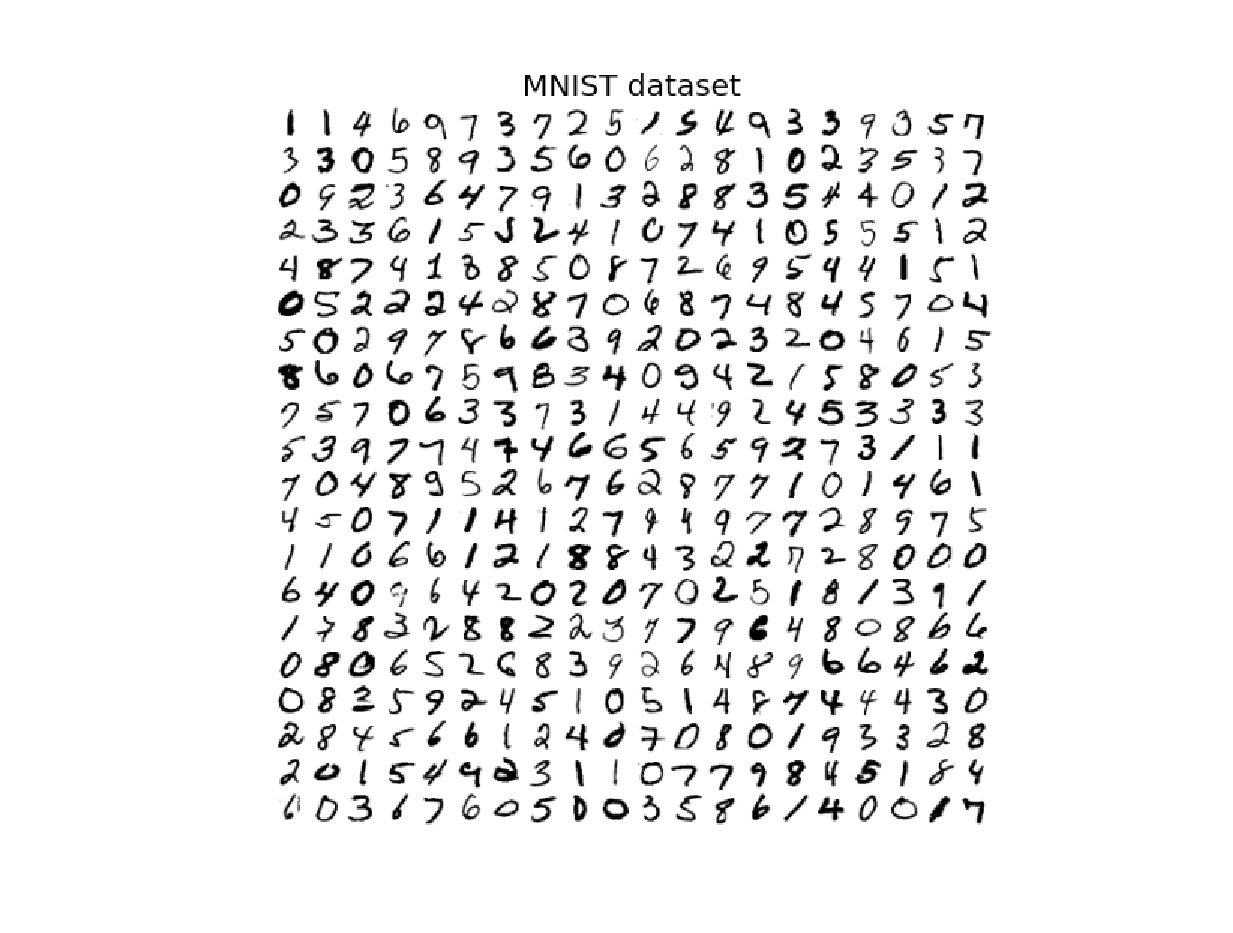
\includegraphics[width=0.4\textwidth]{assets/img/tiled_mnist_nl0.0.eps}
  \caption{MNISTの画像データ}
  \label{fig:plot-mnist}
\end{figure}

また, ノイズを加えた場合の性能変化, ノイズ耐性, 
中間ニューロンの役割, オートエンコーダを利用した画像特徴抽出による
識別性能変化について考察した. 
%%%%%%%%%%%%%%%%%%%%%%%%%%%%%%%%%%%%%%%%%%%%%%%%%%%%%%%%

%%%%%%%%%%%%%%%%%%%%%%%%%%%%%%%%%%%%%%%%%%%%%%%%%%%%%%%%
\section{ニューラルネット学習シミュレーション}
実験に利用したMNISTは, 28 × 28ピクセルのグレースケール手書き数字
画像の70000件のデータセットである. 
データセットを3分割し3分の2を学習データ, 3分の1をテストデータとし, 
以下の様なパラメータに関してモデルの性能を交差検定によって調べた. 

なお, パラメータの検証は以下の順番で行い, 一部を覗いてそれぞれ最良であったものを
次の検証で利用することで, 性能の向上を目指した. 
最初のパラメータ値は, 学習率0.2, 慣性項の係数0, 
隠れ層の数入力の0.1倍, 学習の際のノイズ0とした. 

\begin{itemize}
  \item 学習の際の繰り返し数
  \item 学習率
  \item 慣性項の係数
  \item 隠れ層の数
  \item 学習の際のノイズ率
\end{itemize}

%%%%%%%%%%%%%%%%%%%%%%%%%%%%%%%%%%%%%%%%%%%%%%%%%%%%%%%%

%%%%%%%%%%%%%%%%%%%%%%%%%%%%%%%%%%%%%%%%%%%%%%%%%%%%%%%%
\section{ノイズによる性能変化}
ある確率で画像のピクセル値をランダムな値に変化させるということによって
ノイズをテストデータに発生させ,
予測性能を調べることでノイズの影響を検証した. 

図\ref{fig:noise-0.1}がノイズを10\%,
図\ref{fig:noise-0.25}がノイズを25\%発生させたデータを, 
画像としてプロットしたものである. 

\begin{figure}[htbp]
  \centering
  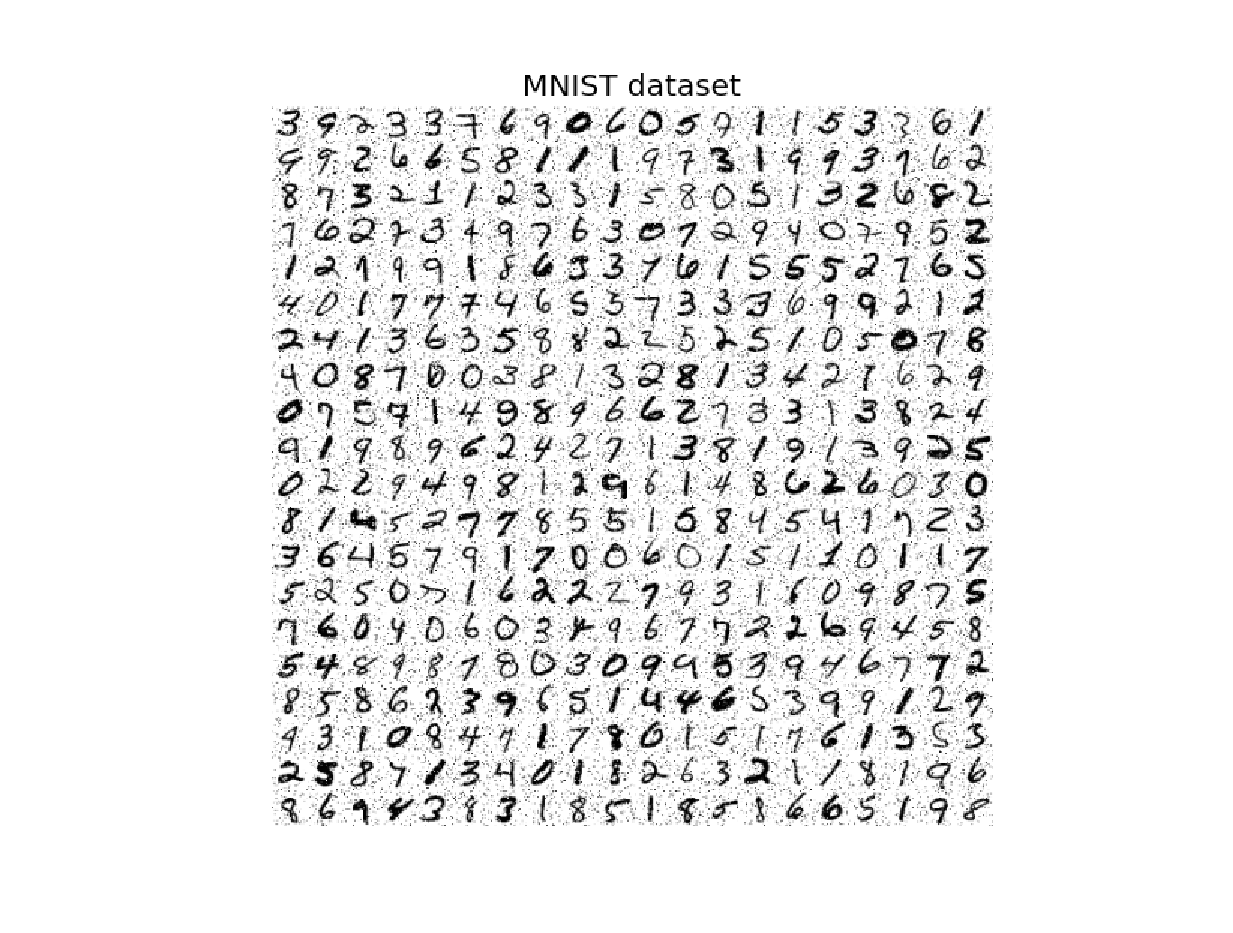
\includegraphics[width=0.4\textwidth]{assets/img/tiled_mnist_nl0.1.eps}
  \caption{ノイズを10\%発生させたデータ}
  \label{fig:noise-0.1}
\end{figure}
\begin{figure}[htbp]
  \centering
  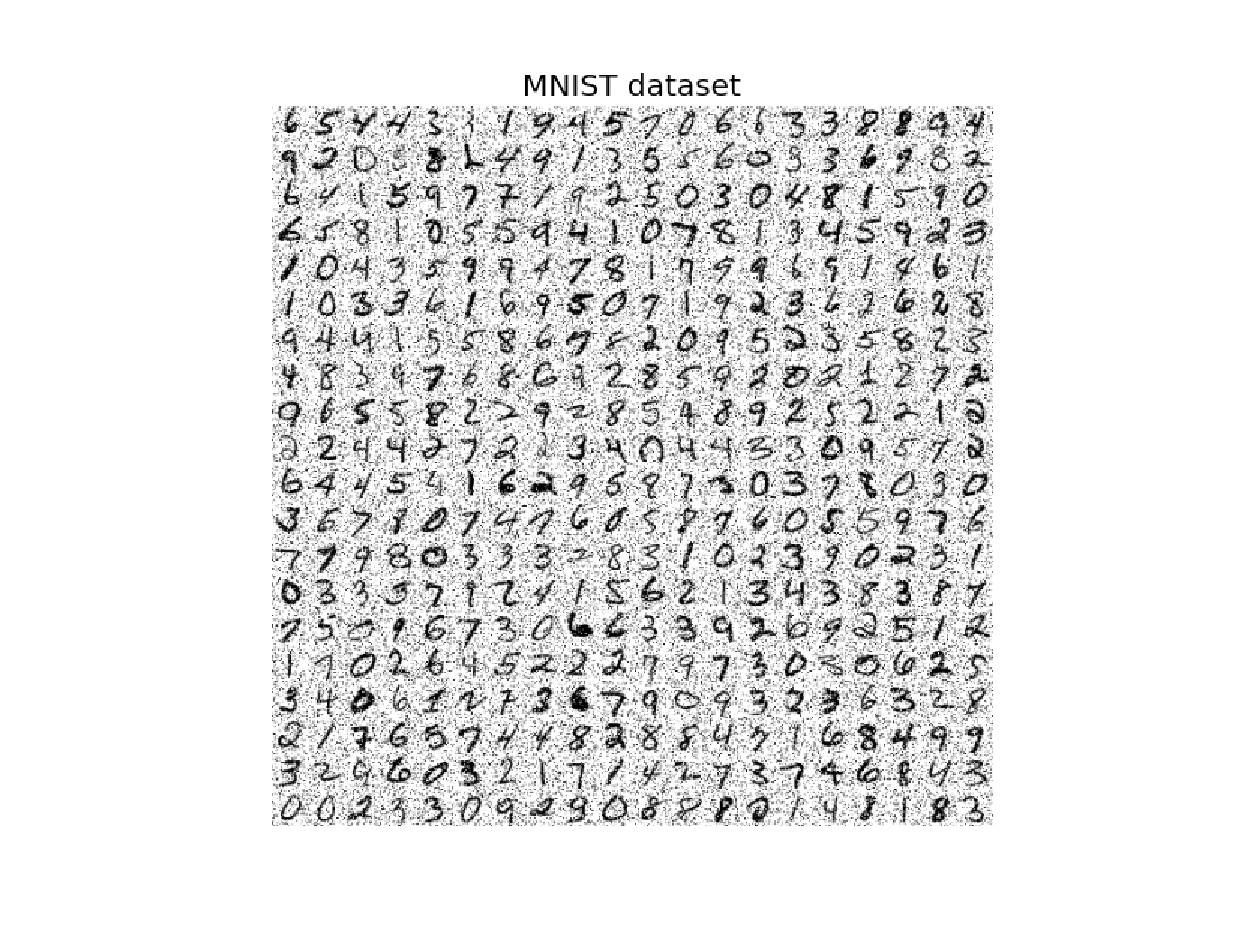
\includegraphics[width=0.4\textwidth]{assets/img/tiled_mnist_nl0.25.eps}
  \caption{ノイズを25\%発生させたデータ}
  \label{fig:noise-0.25}
\end{figure}
%%%%%%%%%%%%%%%%%%%%%%%%%%%%%%%%%%%%%%%%%%%%%%%%%%%%%%%%

%%%%%%%%%%%%%%%%%%%%%%%%%%%%%%%%%%%%%%%%%%%%%%%%%%%%%%%%
% \section{中間層のニューロンの役割}
% 中間層のニューロンの数を変化させ, ニューロン数と識別性能の関係を表した
% のが図\ref{fig:hidden-neuron-role}である. 
% \begin{figure}[htbp]
%   \centering
%   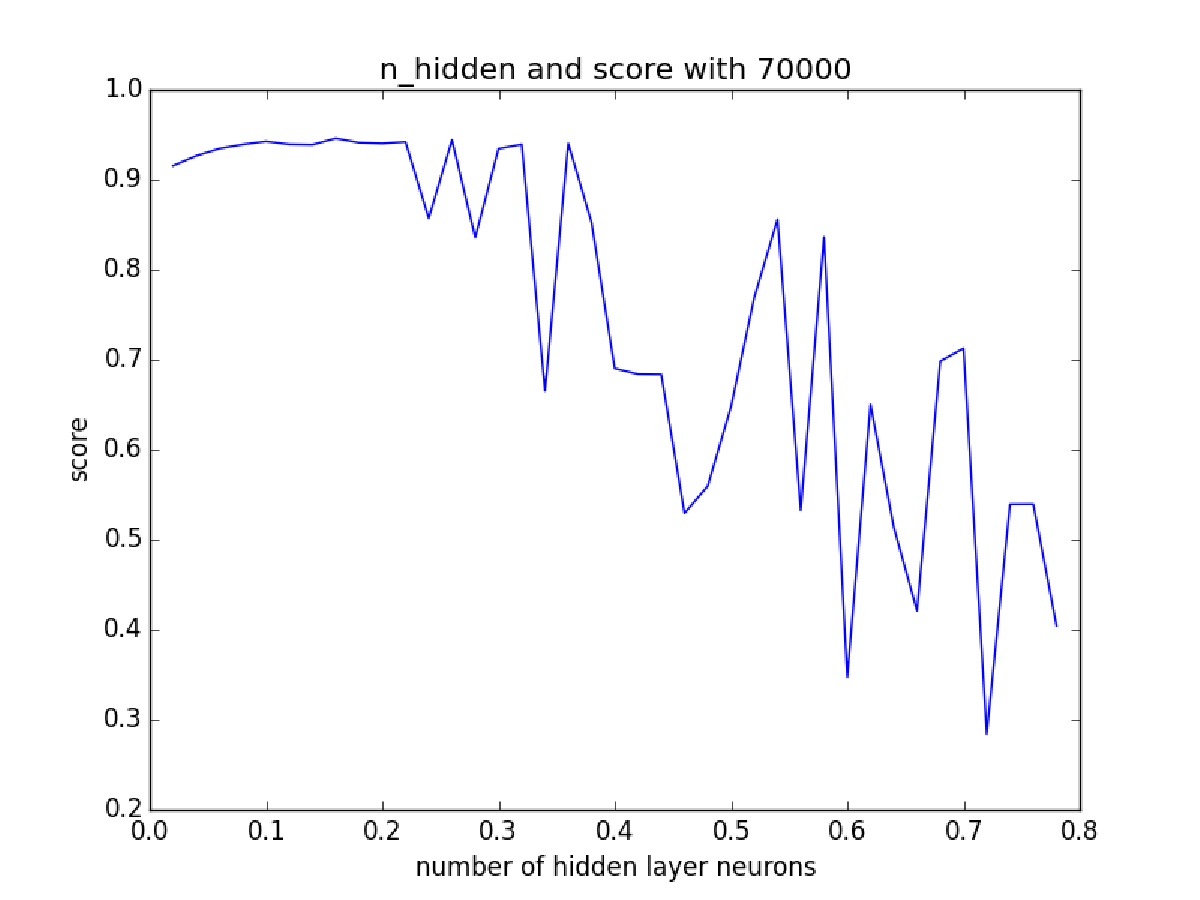
\includegraphics[width=0.4\textwidth]{assets/img/hidden_layer_analyze_mnist_score_70000.pdf}
%   \caption{中間層ニューロン数と識別器の識別性能の関係}
%   \label{fig:hidden-neuron-role}
% \end{figure}
%
% \begin{figure}[htbp] 
%   \centering
%   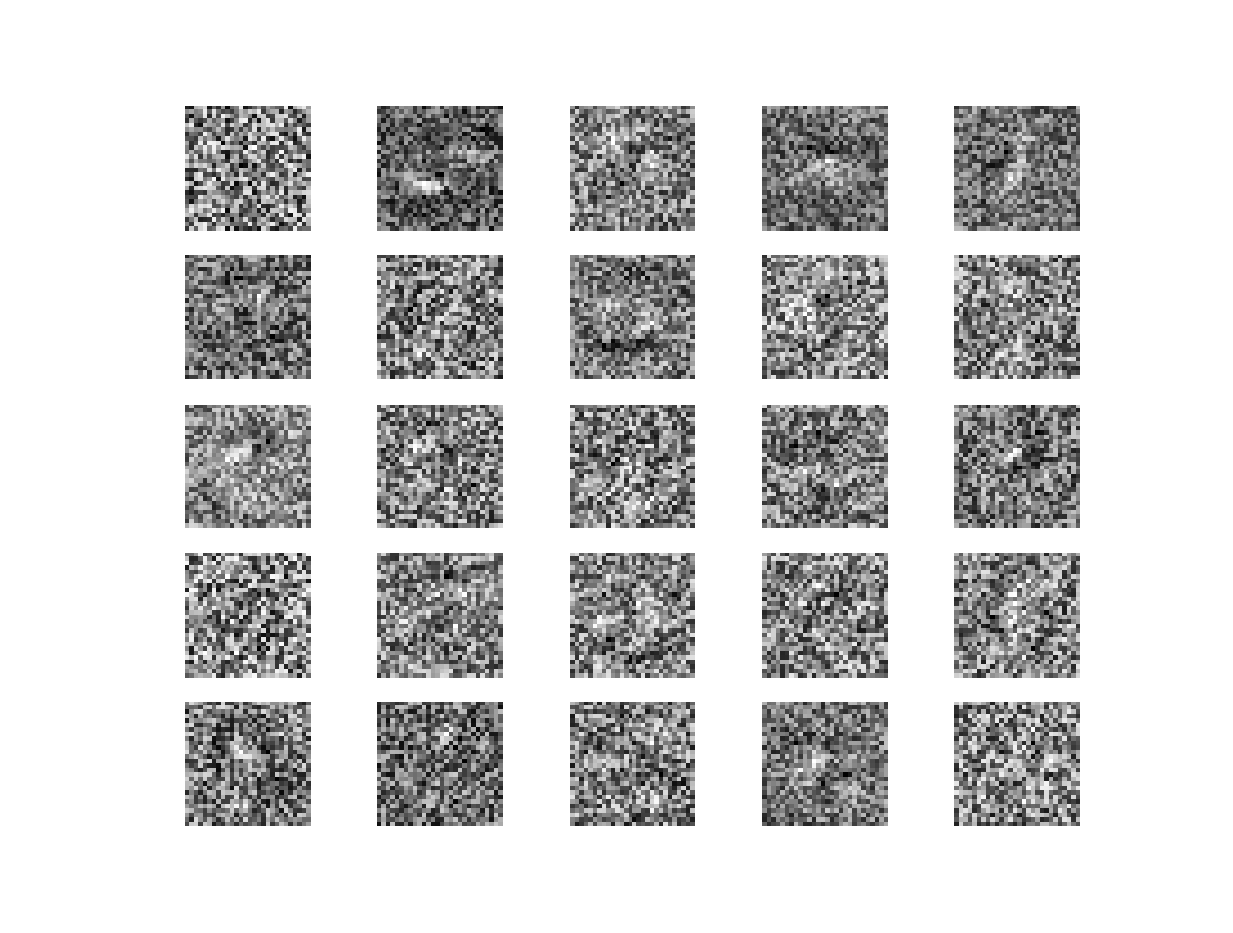
\includegraphics[width=0.4\textwidth]{assets/img/hidden_layer_analyze_mnist_image_nsamp70000_nh0.16.eps}
%   \caption{識別性能が高い場合(中間層0.16)の重み}
%   \label{fig:hidden-layer-analyze-img-0.16}
% \end{figure}
% \begin{figure}[htbp] 
%   \centering
%   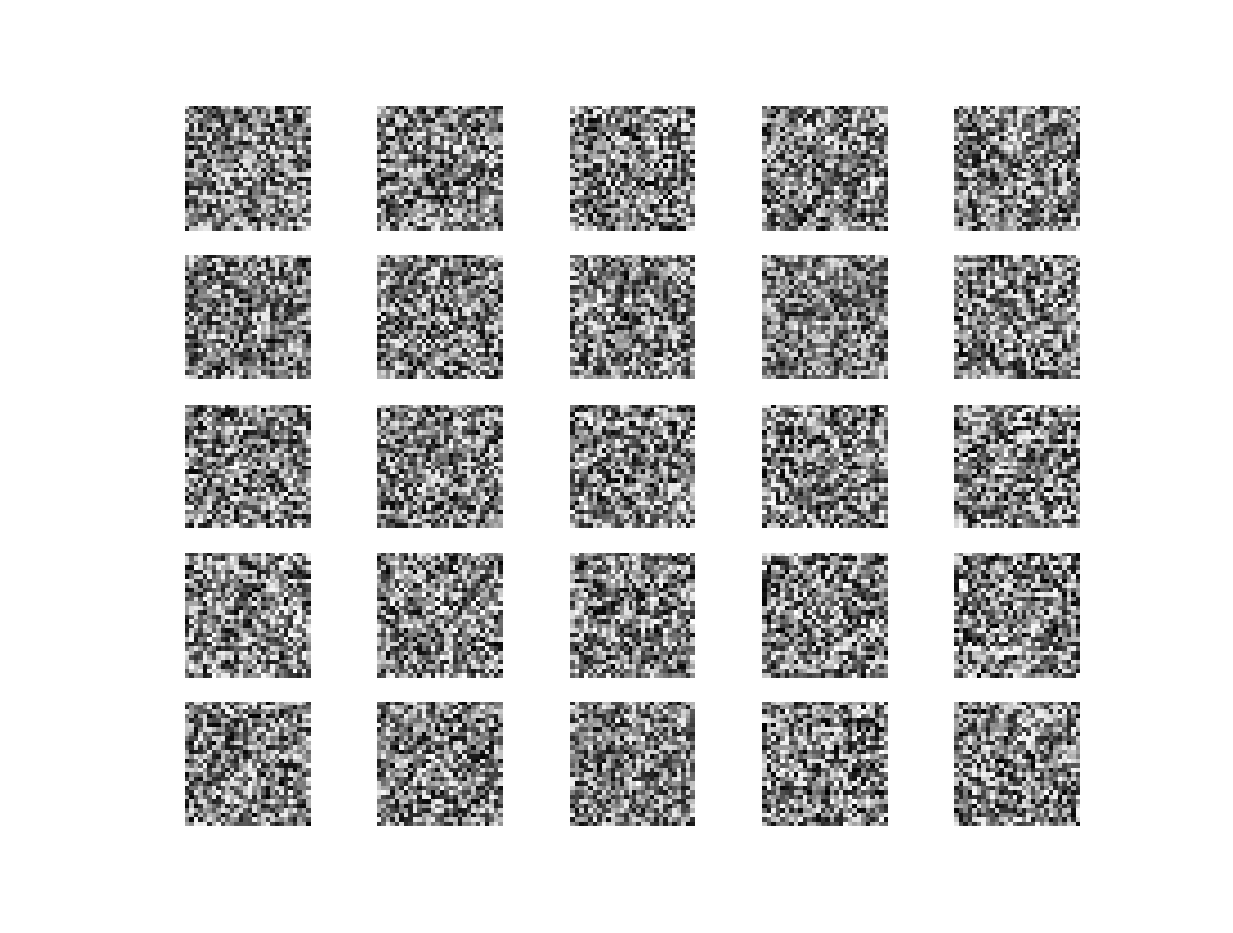
\includegraphics[width=0.4\textwidth]{assets/img/hidden_layer_analyze_mnist_image_nsamp70000_nh0.72.eps}
%   \caption{識別性能が高い場合(中間層0.72)の重み}
%   \label{fig:hidden-layer-analyze-img-0.72}
% \end{figure}
%%%%%%%%%%%%%%%%%%%%%%%%%%%%%%%%%%%%%%%%%%%%%%%%%%%%%%%%
%%%%%%%%%%%%%%%%%%%%%%%%%%%%%%%%%%%%%%%%%%%%%%%%%%%%%%%%
%%%%%%%%%%%%%%%%%%%%%%%%%%%%%%%%%%%%%%%%%%%%%%%%%%%%%%%%
%%%%%%%%%%%%%%%%%%%%%%%%%%%%%%%%%%%%%%%%%%%%%%%%%%%%%%%%
%%%%%%%%%%%%%%%%%%%%%%%%%%%%%%%%%%%%%%%%%%%%%%%%%%%%%%%%


%%%%%%%%%%%%%%%%%%%%%%%%%%
% to insert bibliography %
%%%%%%%%%%%%%%%%%%%%%%%%%%
\begin{thebibliography}{9}
%   \bibitem{inv1} Samuel R.Buss,"Introduction to Inverse Kinematics with Jacobian Transpose,Pseudoinverse and Damped Least Squares methods"
  \bibitem{mnist} Yann LeCun, Corinna Cortes, Christopher J.C. Burges,
    ``MNIST handwritten digit database, Yann LeCun, Corinna Cortes and Chris Burges'',
    http://yann.lecun.com/exdb/mnist/
\end{thebibliography}

%%%%%%%%%%%%%%%%
% end document %
%%%%%%%%%%%%%%%%
\end{document}